\documentclass[sigplan,11pt,nonacm]{acmart}
\settopmatter{printfolios}

\usepackage{booktabs} % For formal tables
\usepackage{subcaption}
\usepackage{tikz}
\usepackage{pgfplots}
\usepackage{pgfplotstable}
\usepackage{hyphenat}
\usepackage{todonotes}
\usepackage[babel]{csquotes}


\begin{document}
\title{Utilizing Parallel Workers: \\LLVM's Vectorization Plan}
\author{Jonas Fritsch}
\affiliation{%
  \institution{Technical University of Munich}
}
\email{jonas.fritsch@tum.de}

\begin{abstract}
Lorem ipsum
\end{abstract}

\maketitle

%%%%%%%%%%%%%%%%%%%%%%%%%%%%%%%%%%%%%%%%%%%%%%%%%%%%%%%%%%%%%%%%%%%%%%%%%%%%%%%%%%%%%%%%%%%%%%%%%%%%%%
%%%%%%%%%%%%%%%%%%%%%%%%%%%%%%%%%%%%%%%%%%%%%%%%%%%%%%%%%%%%%%%%%%%%%%%%%%%%%%%%%%%%%%%%%%%%%%%%%%%%%%
%%%%%%%%%%%%%%%%%%%%%%%%%%%%%%%%%%%%%%%%%%%%%%%%%%%%%%%%%%%%%%%%%%%%%%%%%%%%%%%%%%%%%%%%%%%%%%%%%%%%%%


\section{Introduction}
\label{sec:introduction}
Modern CPUs are often equipped with multiple different vector registers. These registers are nowadays 
as wide as 512 bits, allowing for the processing of multiple data streams at once (SIMD). By 
batching multiple values together in one register, different ISAs like Intel AVX or ARM SVE allow 
the execution of the same instruction for all values in a vector register simultaneously. 
Utilizing this leads to significant performance improvements over the scalar equivalent most of 
the time.

However, manual code vectorization can quickly become time-consuming, especially when
supporting different CPU architectures. Modern compilers aim to automatically transform scalar code
to use vectorization when applicable.

As one of the most widely used compilation frameworks, LLVM~\cite{10.5555/977395.977673} has 
implemented and refined its auto-vectorization over many years. It provides two different 
Vectorizers, one for innermost loops (LoopVectorize) and one for super-word parallelism 
(SLPVectorize)~\cite{llvmvec}.

This system, however, had quite a few limitations, as the loop vectorizer could only handle
innermost loops and neither outer loops, complex control flow, nor non-inlined functions. 
Additionally, while multiple different vectorizations for the same scalar code 
would be possible, the current vectorizers working directly on the LLVM IR could not model
and compare the costs of such different vectorization approaches.

With these limitations in mind, Intel started an ongoing refactorization effort to migrate LLVM's
auto-vectorization pipeline to utilize a more abstract Vectorization Plan 
(VPlan)~\cite{llvmextloopvec,llvmvplan}. The final goal would be to unite LLVM's auto-vectorization
in a single flexible system capable of optimizing SLPs, inner, and nested loops with complex 
control flows. The auto-vectorization pass would create and transform multiple different 
VPlans, each modeling a different vectorization approach, abstracted away from the underlying LLVM IR.
Those VPlans are compared against each other based on a cost model, and finally, the best one, which
might also not vectorize at all, is materialized into the LLVM IR.

LLVM's VPlan is currently being integrated into the existing Loop Vectorizer and is
already modeling most inner loop vectorizations and transformations~\cite{llvmvplanupdate}. 
Vectorization for outer loops is also in development and can be enabled by setting 
the \texttt{-enable-vplan-native-path} flag~\cite{llvmouterloop}. In the future, the plan will 
be to merge both of these loop vectorization paths into one. Merging the existing SLP Vectorizer
with VPlan is also planned.


%%%%%%%%%%%%%%%%%%%%%%%%%%%%%%%%%%%%%%%%%%%%%%%%%%%%%%%%%%%%%%%%%%%%%%%%%%%%%%%%%%%%%%%%%%%%%%%%%%%%%%
%%%%%%%%%%%%%%%%%%%%%%%%%%%%%%%%%%%%%%%%%%%%%%%%%%%%%%%%%%%%%%%%%%%%%%%%%%%%%%%%%%%%%%%%%%%%%%%%%%%%%%
%%%%%%%%%%%%%%%%%%%%%%%%%%%%%%%%%%%%%%%%%%%%%%%%%%%%%%%%%%%%%%%%%%%%%%%%%%%%%%%%%%%%%%%%%%%%%%%%%%%%%%


\section{Background}
\label{sec:background}
In general, vectorization techniques can be separated into different categories:

\subsection{Inner Loop Vectorization}
Innermost loops are loops whose body's control flow does not contain any more loops, bound or unbound.
Vectorization of these loops is more straightforward as the only option to vectorize is over 
the loop's induction variable.

There are various ways to transform the control flow of a loop to accommodate operating on widened
vector registers. Figure~\ref{fig:inner-loop-vec} shows an example of an if-conversion. Some more
examples can also be found in LLVM's Auto-Vectorization Documentation~\cite{llvmvec}.

\begin{figure}
  \centering
  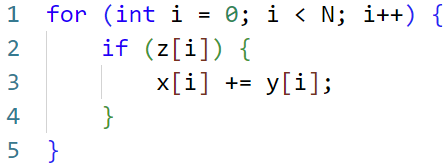
\includegraphics[width=0.35\textwidth]{images/inner-loop-vec.png}
  \caption{A code snippet of a simple loop that would be vectorized over the variable \texttt{i}. 
  The conditional branch would be flattened into a masked addition. The mask would be generated 
  based on \texttt{z[i]}.}
  \label{fig:inner-loop-vec}
\end{figure}

\subsection{Super-Word Parallelism (SLP) Vectorization}
SLP Vectorization vectorizes similar independent instructions. A compiler might have, for example, 
fully unrolled a smaller loop in a previous code simplification pass. The resulting similar scalar 
instructions might then be vectorized later by an SLP vectorizer.

\subsection{Outer Loop Vectorizaton}
Outer loop vectorization focuses on control flow with nested loops. Such loops often present
more challenges for auto-vectorization, as one could vectorize over the outer loop,
inner loop, or a mix of both, representing a hybrid/multi-dimensional vectorization approach. 
Carrying out and comparing costs of such different vectorization approaches can be complex 
and require a flexible system like, for example, VPlans. 

Figure~\ref{fig:outer-loop-vec} shows a nested loop code snippet where vectorization over the
outer loop would be beneficial.

\begin{figure}
  \centering
  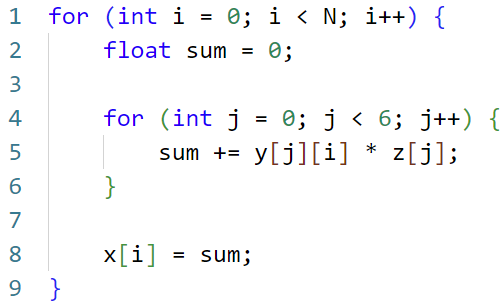
\includegraphics[width=0.39\textwidth]{images/outer-loop-vec.png}
  \caption{A code snippet of a nested loop where it would be beneficial to vectorize over the 
  outer loop. The inner loop has a trip count that is too low (6) to vectorize. Additionally,
  the memory access pattern of \texttt{y} would be consecutive compared to scattered when
  vectorizing over \texttt{i} instead of \texttt{j}.}
  \label{fig:outer-loop-vec}
\end{figure}

\subsection{Function Vectorization}
Function vectorization refers to the vectorization of entire functions. A loop might contain a
non-inlined function call, passing data related to the iteration variable. During auto-vectorization, 
this call could be replaced with a call to a newly constructed function with the same semantic 
control flow but operating on multiple values at once through vector registers instead.

\subsection{Vectorization Similarities}
All of the above-mentioned vectorization techniques can be brought into relation with each other. 
For example, function vectorization can be transformed into loop vectorization by creating a loop 
around the function body and vectorizing it and vice versa. The same applies for SLP Vectorization 
and loop vectorization when unrolling a loop.
 
\subsection{Vectorization Legality}
Not all loops can be vectorized. There are various factors that can ultimately hinder any
vectorization attempts.

Some of the most common vectorization barriers are data dependencies. As the vectorized version
of a code executes for Vectorization Factor (VF) $N$ data streams simultaneously, it inherently changes
the order of operations. To guarantee that the semantics of the code do not change, all
operations on these $N$ data streams must, generally, be independent. The simplest case
where this is not provided is when the $i$-th loop iteration depends on any of the $(i-N)$-th 
previous iterations.

While explicit data dependencies are easier to see, even a simple loop, as in 
Figure~\ref{fig:inner-loop-vec}, could carry an implicit dependency in line 3, if
the \texttt{x} and \texttt{y} point to overlapping memory regions (pointer aliasing).

Not all data dependencies directly hinder any vectorization. One exception can 
sometimes be made for reduction idioms, as seen in the inner loop in 
Figure~\ref{fig:outer-loop-vec}, where \texttt{sum} would be a reduction variable.

Additionally, the control flow should be primarily straight-line code. While most if-else 
constructs can be flattened to always execute both branches along with masking, the same is not 
valid for switch-case statements or too complex control flows.

\subsection{Vectorization Costs}
While it may not be legal to vectorize a given control flow, the vectorized code sometimes 
performs worse than its scalar equivalent.

Some control flow transformations that seem beneficial at compile time might reveal a performance
bottleneck at runtime. Considering the code snippet from Figure~\ref{fig:inner-loop-vec}, it might
be that almost all \texttt{z[i]} evaluate to false at runtime. The branch predictor of a CPU
would then be able to guess the correct branch in the scalar code. The vectorized version would
always load the \texttt{y[i]} into memory only for the addition to be masked away. Different 
approaches to avoid such runtime penalties are branch-on-superword-condition code 
(BOSCC)~\cite{10.5555/1299042.1299055,llvmboscc} or active-lane 
consolidation (ALC)~\cite{10.1007/s11227-022-04359-w,10.5555/3615924.3615932}.

Some vector instructions can be costly on most CPUs. Examples are gather, scatter, shuffle,
and permutation instructions. Control flow with many non-adjacent memory loads/stores or 
operations that combine different vector elements, such as reductions, can decrease vectorization 
performance.

Additionally, the vectorized code size will always be larger than the scalar equivalent. This is
due to many factors: (1) The transformed control flow often includes more instructions.
(2) As the loop trip count might not be a perfect multiple of the vectorization factor, a scalar
epilogue/remainder of the loop might be used to handle the tail iterations. (3) Various runtime
checks might be inserted throughout the vectorized control flow to handle, for example, pointers 
to overlapping memory regions, in which case the scalar version of the loop is executed.



%%%%%%%%%%%%%%%%%%%%%%%%%%%%%%%%%%%%%%%%%%%%%%%%%%%%%%%%%%%%%%%%%%%%%%%%%%%%%%%%%%%%%%%%%%%%%%%%%%%%%%
%%%%%%%%%%%%%%%%%%%%%%%%%%%%%%%%%%%%%%%%%%%%%%%%%%%%%%%%%%%%%%%%%%%%%%%%%%%%%%%%%%%%%%%%%%%%%%%%%%%%%%
%%%%%%%%%%%%%%%%%%%%%%%%%%%%%%%%%%%%%%%%%%%%%%%%%%%%%%%%%%%%%%%%%%%%%%%%%%%%%%%%%%%%%%%%%%%%%%%%%%%%%%


\section{LLVM's Vectorization Plan}
\label{sec:vplan}

\subsection{History}
LLVM implements two different vectorizers for auto-vectorization, LoopVectorize (LV)
and SLPVectorize. These vectorizers are a part of LLVM's middle-end and run after module 
simplification has taken place. As VPlan has not yet been integrated into SLP-Vectorization 
we will only focus on explaining the original LoopVectorize structure.

LoopVectorize was designed to focus only on vectorization of innermost loops~\cite{llvmintrvplan}. 
When starting with a initial scalable loop in IR it would first run a legality phase to check 
whetever and how it is legal to vectorize the loop. This phase would produce artifacts/maps like if 
and what runtime aliasing checks would be required. Then the cost model ran next, creating more 
artifacts based on the scalar IR and legality artifacts. These cost model artifacts would 
associate different vectorization factors with a cost. Lastly the transformation phase would 
vectorize the underlying IR in one go based on all the produced artifacts.

However, this rigid flow of LoopVectorize was a problem. Extending LV to include outer loop 
and nested loop vectorizations would have been very challenging, as LV was designed to flatten a
loops control flow into a single basic block. Producing and considering more and 
more artifacts when trying to transform the scalar loop into a vectorized one all at once did also 
not scale well.

As a potential solution Intel proposed a long-term effort to refactor LLVM's whole auto-vectorization
using a system called Vectorization Plan (VPlan)~\cite{llvmextloopvec}.

The goal was to unite any auto-vectorization systems (SLP, Inner-/Outer-Loop) into a single flexible
system~\cite{llvmintrvplan,llvmvplanstate}, as seen in Figure~\ref{fig:vplan-future}. This system would use VPlans to represent different 
vectorization approaches, abstracted away from the underlying IR. Each VPlan would be able to 
calculate its cost and transform itself to modify the final IR. At first the Legality 
phase (yellow) would check if the scalar code would be legal to vectorize at all and if so initial 
VPlans would be constructed. In the following Planning phase (magenta) these initial VPlans would 
be optimized using various VPlan-to-VPlan transformations. Those transformations would be supervised 
by the VPlan's cost model. Finally, the best VPlan would be chosen and materialized/executed, 
modifying the underlying IR. The best VPlan might also be to not vectorize at all (VF $=1$).

\begin{figure}
  \centering
  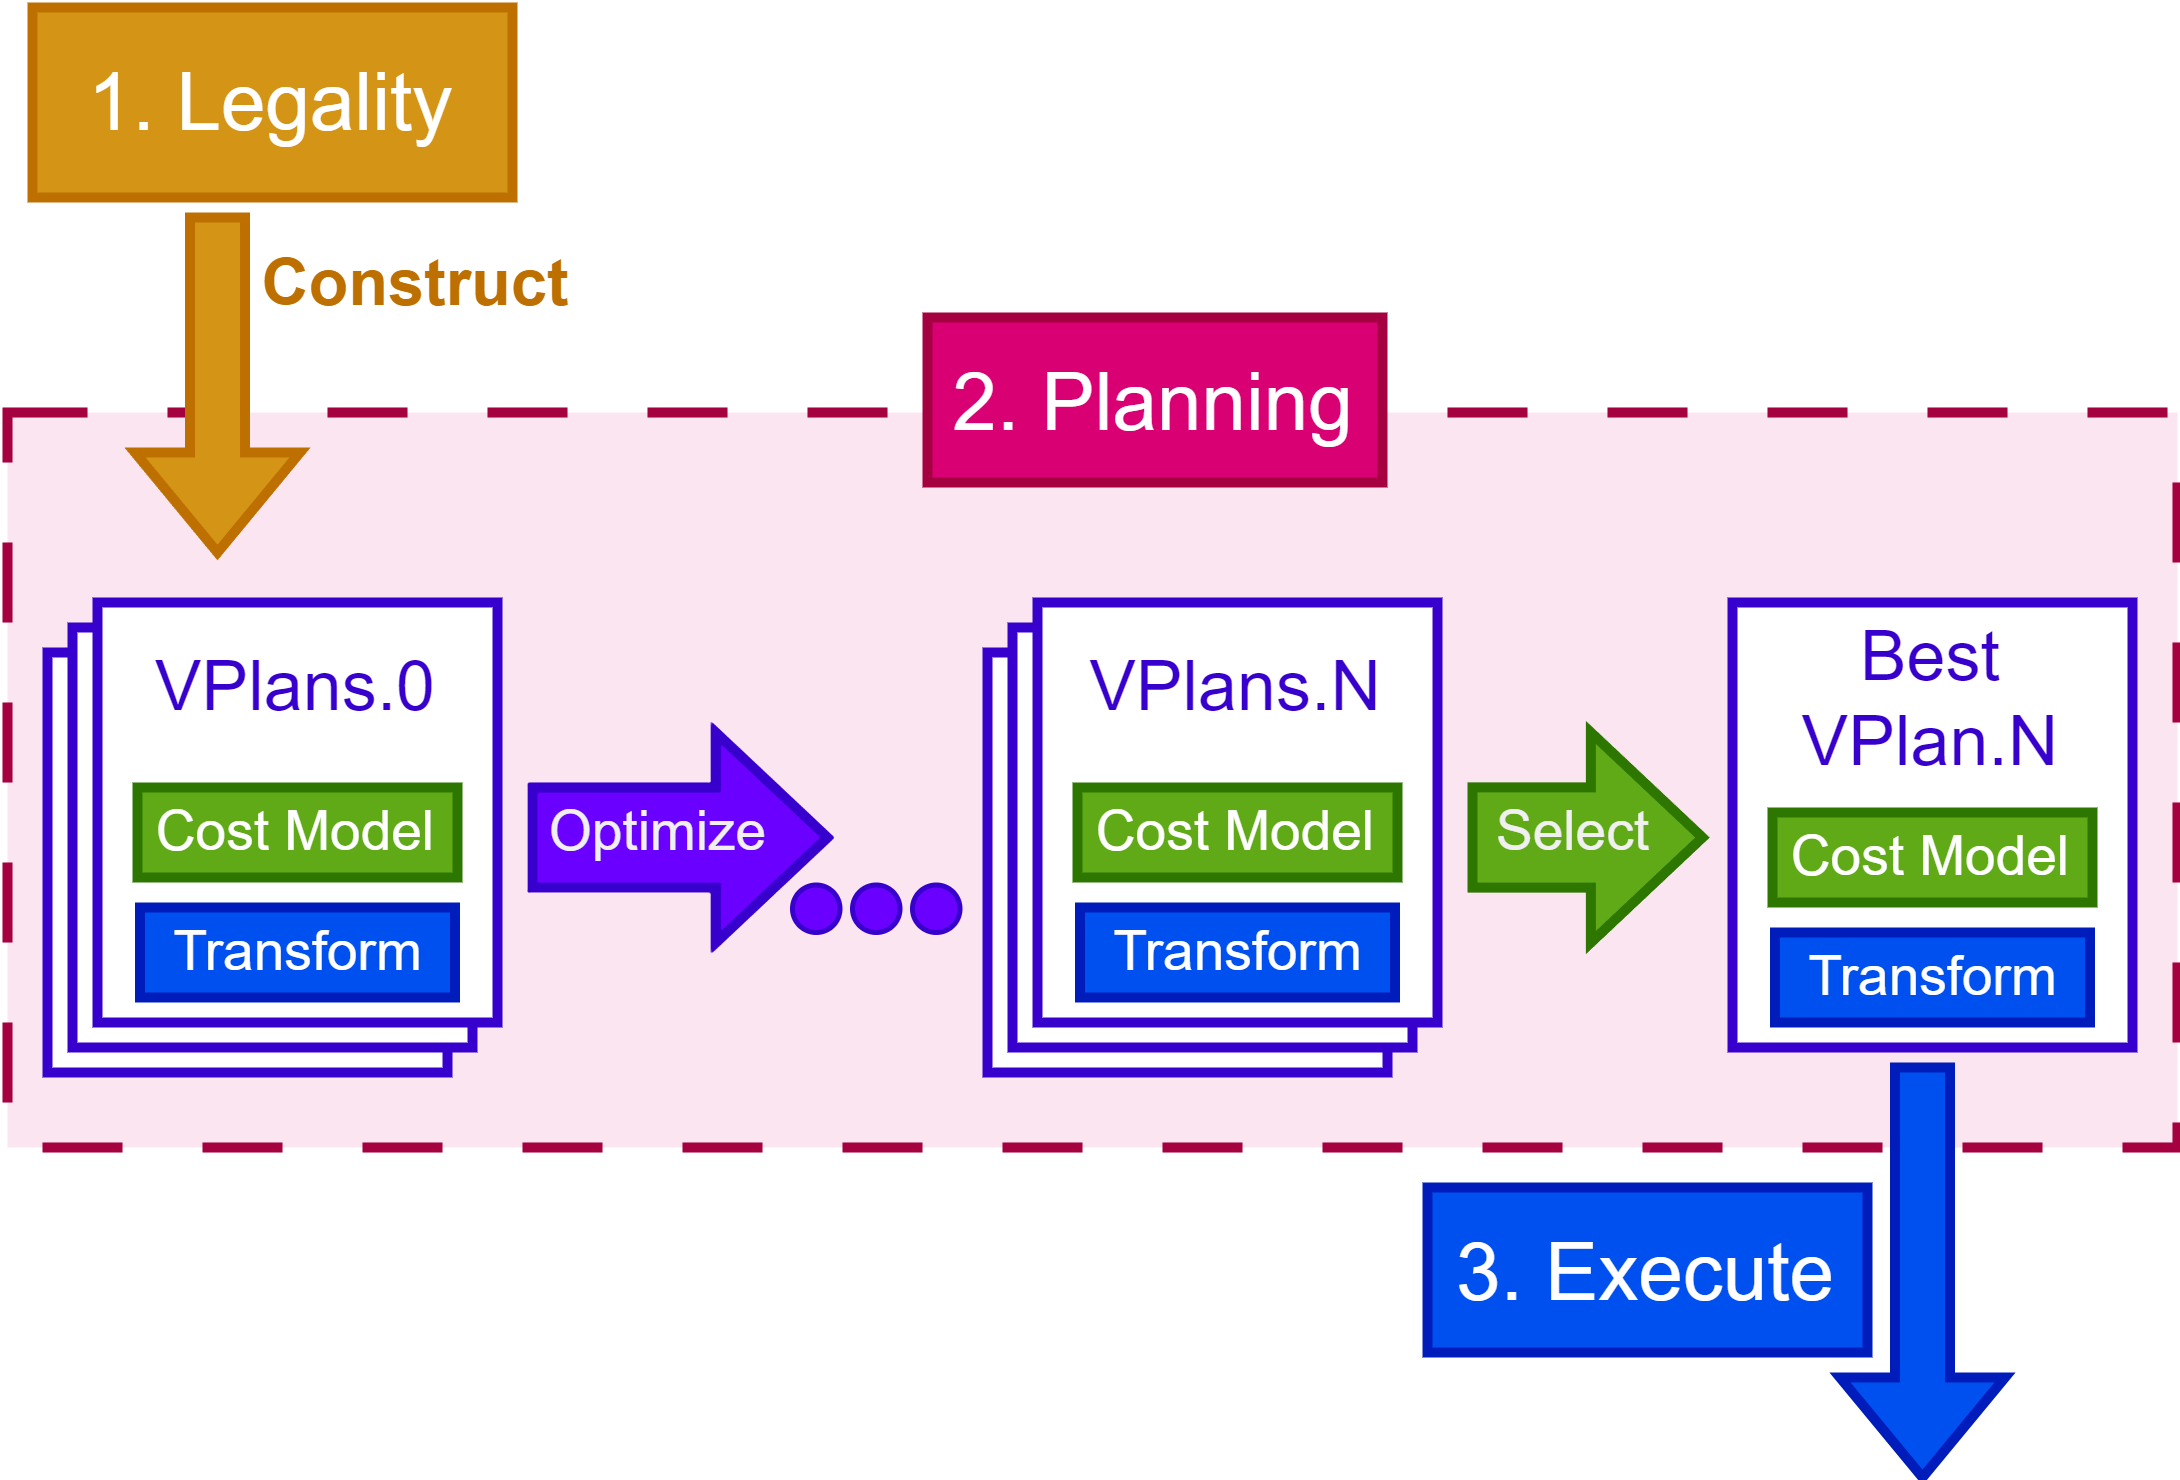
\includegraphics[width=0.475\textwidth]{images/vplan-future.png}
  \caption{The planned future architecture for VPlan. The VPlan optimization would
  work as iteratively applying VPlan-to-VPlan transformations.}
  \label{fig:vplan-future}
\end{figure}

\subsection{Current State of VPlan}

In its current state (LLVM 19.1.4) VPlan is deeply integrated into LV. 


\begin{figure*}[ht!]
  \centering
  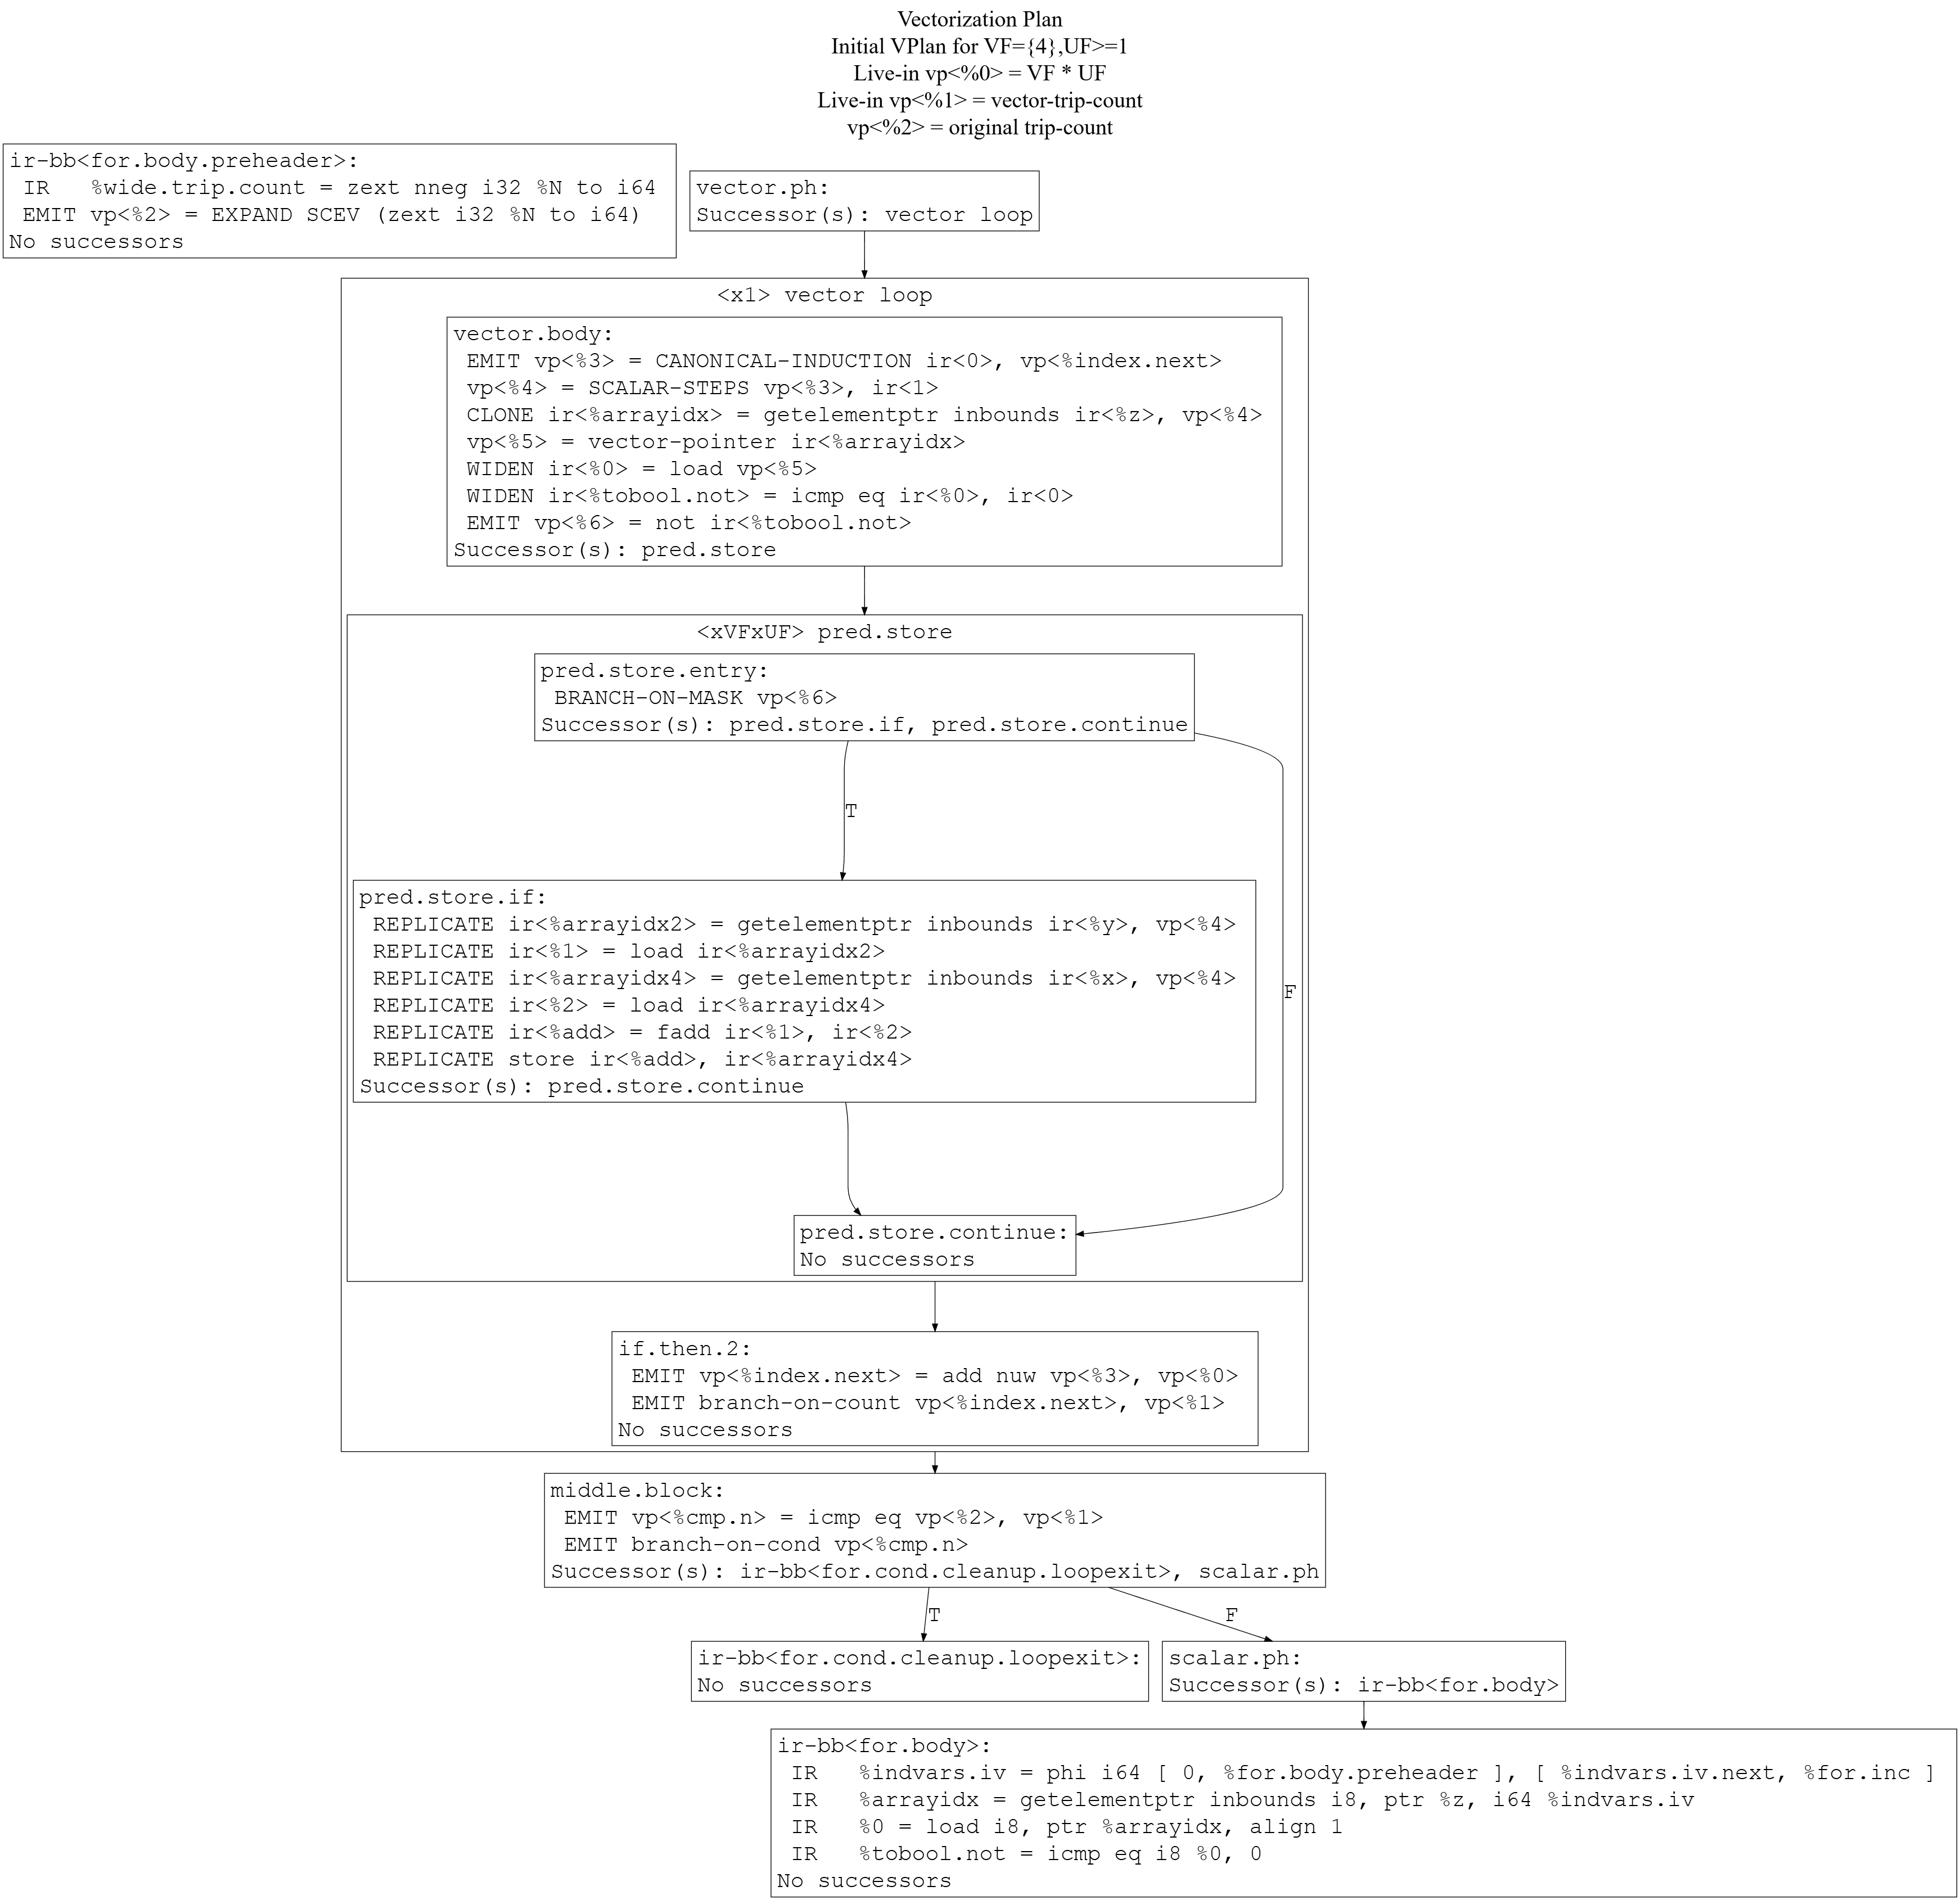
\includegraphics[width=\textwidth]{images/inner-loop-vplan-hcfg.png}
  \caption{Hierarchical CFG of a VPlan modelling the vectorized version of the loop in 
  Figure~\ref{fig:inner-loop-vec}.}
  \label{fig:inner-loop-vplan-hcfg}
\end{figure*}

\subsection{Future of VPlan}
Many of the VPlan internals and systems surrounding it are still in active development. To stay
up-to-date with the latest developments regarding auto-vectorization in LLVM one can follow the 
Community Forum\footnote{\url{https://discourse.llvm.org/c/ir-optimizations/loop-optimizations/62}} or
attend the monthly online 
meetings\footnote{\url{https://discourse.llvm.org/t/monthly-vectorizer-online-sync-up/78978/3}}.

\subsubsection{General VPlan and Integration with LV}
The main effort of setting up the VPlan structure and integrating it first into LV has seen
tremendous effort over the last years. Florian Hahn presented future directions for 
VPlan~\cite{llvmvplanupdate}, which mostly evolve around transforming more LV-based decisions into
explicit VPlan-to-VPlan transformations. Additionally, a lot of cost model related decisions 
still end up being influenced by the old legacy LV cost model, however, transition to a VPlan-based 
cost model has already started.

\subsubsection{Outer Loop Vectorization}
Development around outer loop vectorization has slowed down a bit as focus shifted more onto VPlan
internals and integration into LV. The inner loop path and outer loop path are currently still
seperated by the experimental \texttt{-enable-vplan-native-path} flag. Further developing the 
outer loop path and eventually merging it with the innermost loop path is planned.

\subsubsection{Merging with SLP Vectorize}
Merging the existing SLP Vectorizer with the current VPlan infrastructure is in the early phase
of planning.

\subsubsection{Function Vectorization}
As far as we now there is currently no active development for whole-function vectorization in the
llvm-project's upstream yet.


%%%%%%%%%%%%%%%%%%%%%%%%%%%%%%%%%%%%%%%%%%%%%%%%%%%%%%%%%%%%%%%%%%%%%%%%%%%%%%%%%%%%%%%%%%%%%%%%%%%%%%
%%%%%%%%%%%%%%%%%%%%%%%%%%%%%%%%%%%%%%%%%%%%%%%%%%%%%%%%%%%%%%%%%%%%%%%%%%%%%%%%%%%%%%%%%%%%%%%%%%%%%%
%%%%%%%%%%%%%%%%%%%%%%%%%%%%%%%%%%%%%%%%%%%%%%%%%%%%%%%%%%%%%%%%%%%%%%%%%%%%%%%%%%%%%%%%%%%%%%%%%%%%%%


\section{Related Work}
\label{sec:relatedwork}
Lorem ipsum


%%%%%%%%%%%%%%%%%%%%%%%%%%%%%%%%%%%%%%%%%%%%%%%%%%%%%%%%%%%%%%%%%%%%%%%%%%%%%%%%%%%%%%%%%%%%%%%%%%%%%%
%%%%%%%%%%%%%%%%%%%%%%%%%%%%%%%%%%%%%%%%%%%%%%%%%%%%%%%%%%%%%%%%%%%%%%%%%%%%%%%%%%%%%%%%%%%%%%%%%%%%%%
%%%%%%%%%%%%%%%%%%%%%%%%%%%%%%%%%%%%%%%%%%%%%%%%%%%%%%%%%%%%%%%%%%%%%%%%%%%%%%%%%%%%%%%%%%%%%%%%%%%%%%


\section{Summary and Future Work}
\label{sec:summary}
Lorem ipsum


%%%%%%%%%%%%%%%%%%%%%%%%%%%%%%%%%%%%%%%%%%%%%%%%%%%%%%%%%%%%%%%%%%%%%%%%%%%%%%%%%%%%%%%%%%%%%%%%%%%%%%

\bibliographystyle{ACM-Reference-Format}
\bibliography{paper} % read paper.bib file

\end{document}
